% ============================================================================
%  Informe tecnico - Proyecto 2: Sistema Multimodal de Recuperacion y Busqueda
%  CS2042 Bases de Datos II - UTEC - Ciclo 2026-1
%
%  Compilar con:  pdflatex informe.tex   (dos veces, para el indice y refs)
%  Las figuras salen de ../backend/experiments/results/ (generadas por los
%  scripts de benchmark). Si compilas desde otra carpeta, ajusta \graphicspath.
% ============================================================================
\documentclass[11pt,a4paper]{article}

\usepackage[utf8]{inputenc}
\usepackage[T1]{fontenc}
% es-noshorthands: desactiva los atajos de babel ("<", ">", comillas) que
% chocan con el codigo y con operadores como <=> de pgvector.
\usepackage[spanish,es-noshorthands]{babel}
\usepackage{lmodern}
\usepackage{graphicx}
\usepackage{booktabs}
\usepackage{array}
\usepackage{amsmath}
\usepackage{listings}
\usepackage{xcolor}
\usepackage{geometry}
\usepackage{caption}
\usepackage[hidelinks]{hyperref}

\geometry{margin=2.5cm}
\graphicspath{{../backend/experiments/results/}}

% Estilo sobrio para los bloques de codigo/SQL.
\definecolor{codegray}{gray}{0.95}
\lstset{
  basicstyle=\ttfamily\small,
  backgroundcolor=\color{codegray},
  breaklines=true,
  frame=single,
  framesep=4pt,
  columns=fullflexible,
  keepspaces=true,
  showstringspaces=false,
}

\title{\textbf{Sistema Multimodal de Recuperación y Búsqueda}\\[2pt]
\large Informe técnico --- Proyecto 2}
\author{Curso: Base de Datos II (CS2042) --- UTEC --- Ciclo 2026-1}
\date{\today}

\begin{document}
\maketitle

\begin{abstract}
\noindent
Implementamos un motor de recuperación por similitud que aplica \emph{la misma}
arquitectura --- \textit{split} $\rightarrow$ extractor $\rightarrow$ codebook
$\rightarrow$ índice invertido $\rightarrow$ búsqueda por coseno --- a tres
modalidades: texto (letras de canciones), imagen (productos de moda) y audio
(pistas musicales). Sobre él construimos dos aplicaciones y lo comparamos contra
las técnicas nativas de PostgreSQL: \texttt{GIN} full-text para texto y
\texttt{pgvector} (con índice \texttt{HNSW}) para vectores. El informe describe
la arquitectura, los datasets, la implementación por módulo y una evaluación
experimental de latencia, throughput, \textit{recall} y memoria que cuantifica
los \textit{trade-offs} entre nuestro índice invertido y los índices nativos.
\end{abstract}

\tableofcontents

% ---------------------------------------------------------------------------
\section{Descripción del sistema y arquitectura}

El objetivo del proyecto es demostrar que distintos tipos de contenido pueden
indexarse y recuperarse con \emph{un mismo paradigma}. En lugar de un motor por
modalidad, tenemos un solo pipeline y cada modalidad solo cambia dos piezas: el
\textbf{extractor} de características y el \textbf{codebook}. Todo lo demás
--- índice invertido, búsqueda por coseno, persistencia --- se reutiliza tal
cual.

\begin{center}
\fbox{\texttt{CONTENIDO $\rightarrow$ SPLIT $\rightarrow$ EXTRACTOR
$\rightarrow$ CODEBOOK $\rightarrow$ ÍNDICE INVERTIDO $\rightarrow$ BÚSQUEDA}}
\end{center}

\begin{table}[h]
\centering
\caption{Adaptación de cada etapa a las tres modalidades.}
\begin{tabular}{@{}p{2.4cm}p{3.5cm}p{3.5cm}p{3.5cm}@{}}
\toprule
\textbf{Etapa} & \textbf{Texto} & \textbf{Imagen} & \textbf{Audio} \\
\midrule
Split      & párrafos / estrofas & imagen del producto & ventanas de 3\,s \\
Extractor  & tokens (nltk) & SIFT (128-d) & MFCC (40-d) \\
Codebook   & top-$k$ palabras ($k{=}1024$) & K-Means ($k{=}512$) & K-Means ($k{=}128$) \\
Ponderación& $\log(1{+}\mathrm{tf})\cdot\mathrm{idf}$ & ídem (visual words) & ídem (acoustic words) \\
Índice     & SPIMI $\rightarrow$ invertido & el mismo índice & el mismo índice \\
Búsqueda   & coseno & el mismo coseno & el mismo coseno \\
\bottomrule
\end{tabular}
\end{table}

El corazón de la búsqueda es \texttt{search\_sparse}: recibe el histograma
disperso de una consulta y acumula el puntaje coseno recorriendo únicamente los
\textit{chunks} que comparten alguna \textit{codeword} con la consulta
(\textit{accumulator pattern}). No le importa la modalidad de origen, y esa es
justamente la razón de que la arquitectura sea agnóstica.

\paragraph{Aplicaciones implementadas.} El backend soporta tres de las ideas
sugeridas (el enunciado pide al menos dos):
\begin{enumerate}
  \item \textbf{Búsqueda Visual E-commerce} (imagen): el usuario sube una foto y
        obtiene los productos más similares.
  \item \textbf{Búsqueda Musical} (texto + audio): buscar canciones por letra
        (full-text) o por similitud acústica.
  \item \textbf{Consola SQL multimodal}: un mini-lenguaje que unifica las
        búsquedas de las tres modalidades desde una sola interfaz.
\end{enumerate}

% ---------------------------------------------------------------------------
\section{Dataset utilizado y características}

\begin{itemize}
  \item \textbf{Música (texto + audio).} \textit{Audio features and lyrics of
        Spotify songs} (Kaggle) para las letras: \textbf{18\,454} canciones con
        letra, multilingüe (mayoría inglés, algo de español). Para audio,
        \textit{GTZAN} con \texttt{features\_3\_sec.csv}: cada pista se parte en
        ventanas de 3\,s y se describe con 20 MFCC (media + varianza $= 40$
        características por ventana).
  \item \textbf{Imagen.} \textit{Fashion Product Images (Small)} (Kaggle):
        \textbf{44\,326} imágenes de productos de moda. Cada producto aporta un
        conjunto de descriptores SIFT que se resumen en un histograma
        Bag-of-Visual-Words.
\end{itemize}

Los datasets no se versionan en el repositorio (son pesados; van en
\texttt{.gitignore}) y se descargan de Kaggle a \texttt{data/raw/}. El
\textit{ingest} acepta \texttt{.csv}, \texttt{.json} y \texttt{.parquet} y mapea
columnas por alias, de modo que el dataset es intercambiable.

\paragraph{Requisitos.} \textit{Funcionales}: búsqueda por letra, por imagen y
por similitud acústica; retorno de top-$N$ con puntaje. \textit{No funcionales}:
latencia interactiva (decenas de ms), bajo consumo de memoria del índice propio
y persistencia en PostgreSQL.

% ---------------------------------------------------------------------------
\section{Detalles de implementación por módulo}

\subsection{Split}
\begin{itemize}
  \item \textbf{Texto} (\texttt{split/paragraph.py}): separa por dobles saltos
        de línea (una estrofa = un \textit{chunk}); si no hay, cae a un chunk
        único.
  \item \textbf{Imagen}: cada producto es un objeto; los ``chunks'' son sus
        descriptores locales SIFT.
  \item \textbf{Audio} (\texttt{split/audio\_window.py}): ventanas deslizantes
        de 3\,s tomadas directamente de las filas del CSV de GTZAN.
\end{itemize}

\subsection{Extractor}
\begin{itemize}
  \item \textbf{Texto} (\texttt{codebook/text\_norm.py}): tokenización con
        expresión regular $\rightarrow$ minúsculas $\rightarrow$ eliminación de
        \textit{stopwords} (español + inglés, vía nltk) $\rightarrow$
        \textit{stemming} con \texttt{SnowballStemmer}. Es la única puerta de
        entrada del texto: tanto el ingest como las consultas pasan por
        \texttt{tokens()}.
  \item \textbf{Imagen} (\texttt{extractor/sift.py}): SIFT de OpenCV,
        descriptores de 128 dimensiones por \textit{keypoint}; la imagen se
        estandariza de tamaño para igualar la escala. Adicionalmente
        (\texttt{extractor/color.py}) se extrae un histograma de color HSV de 32
        \textit{bins} (16 tono + 8 saturación + 8 valor), ignorando el fondo
        casi blanco del dataset.
  \item \textbf{Audio} (\texttt{extractor/mfcc.py}): 20 coeficientes MFCC;
        acepta tanto el vector ya calculado del CSV como audio crudo procesado
        con \texttt{librosa}.
\end{itemize}

\subsection{Codebook}
\begin{itemize}
  \item \textbf{Texto} (\texttt{codebook/linguistic.py}): las $k$ palabras
        (stems) más frecuentes de toda la colección conforman el diccionario.
  \item \textbf{Imagen y audio} (\texttt{codebook/kmeans.py}):
        \texttt{MiniBatchKMeans} sobre todos los descriptores de la colección;
        los $k$ centroides son las ``palabras visuales'' / ``acústicas''.
\end{itemize}

En las tres modalidades el histograma se pondera con \textbf{TF-IDF} --- usando
TF sublineal $\log(1+\mathrm{tf})$ --- y luego se normaliza en $L_2$. El TF
sublineal evita que una \textit{codeword} muy repetida (el coro de una canción,
una textura repetitiva) domine el histograma por pura cantidad; el IDF penaliza
las que aparecen en casi todos los ítems (poco discriminativas):
\begin{equation}
  w_{i} = \log\!\big(1+\mathrm{tf}_{i}\big)\cdot \mathrm{idf}_{i},
  \qquad
  \mathrm{idf}_{i} = \log_{10}\!\frac{N}{\mathrm{df}_{i}},
\end{equation}
donde $N$ es el número de ítems y $\mathrm{df}_i$ en cuántos aparece la
\textit{codeword} $i$. Con la normalización $L_2$, la similitud coseno entre dos
histogramas se reduce a su producto punto.

\paragraph{Tamaño del codebook ($k$).} Es la perilla central del \textit{trade-off}
calidad/costo: con $k$ chico la cuantización confunde contenidos distintos
(falsos positivos); con $k$ grande el vocabulario discrimina más, a costa de
memoria e indexación. Usamos $k=1024$ palabras para texto (18\,454 canciones),
$k=512$ \textit{visual words} para imagen ($\sim$965\,000 descriptores SIFT) y
$k=128$ \textit{acoustic words} para audio, respetando el tope de 2\,000
dimensiones que indexa el HNSW de pgvector.

\paragraph{Fusión de color (imagen).} El histograma final de un producto
concatena la parte visual (SIFT) y la de color, ponderadas de modo que el
vector siga siendo unitario:
\[
  h = \big[\,\sqrt{1-\alpha}\;\text{BoVW}\;\big\Vert\;\sqrt{\alpha}\;\text{color}\,\big],
\]
con lo que el coseno resulta un promedio ponderado entre similitud de forma
(SIFT) y de color, controlado por $\alpha$.

\subsection{Índice invertido (SPIMI)}
El índice invertido mapea cada \textit{codeword} a la lista de \textit{chunks}
que la contienen, con su peso. Para texto se construye con \textbf{SPIMI}
(\textit{Single-Pass In-Memory Indexing}, \texttt{index/spimi.py}):

\begin{enumerate}
  \item Recorre los \textit{chunks} en una sola pasada acumulando \textit{postings}
        en memoria.
  \item Cuando el bloque llena \texttt{block\_size}, lo vuelca a disco
        \emph{ordenado por} \texttt{word\_idx} y libera memoria.
  \item Al final hace un \textit{k-way merge} de los bloques
        (\texttt{heapq.merge}) para producir el índice final.
\end{enumerate}

Este diseño escala a colecciones que no caben en RAM (ajustando
\texttt{block\_size}). El mismo indexador se usa para imagen y audio, ya que a
esa altura del pipeline todo son histogramas dispersos.

\subsection{Búsqueda por coseno}
\texttt{search\_sparse} (\texttt{search/similarity.py}) implementa el
\textit{CosineScore} con acumuladores:
\[
  \mathrm{score}(c) = \sum_{i \in q\cap c} q_i\, d_{c,i},
  \qquad
  \cos(q,c) = \frac{\mathrm{score}(c)}{\lVert q\rVert\,\lVert d_c\rVert}.
\]
Solo se tocan los documentos que comparten alguna \textit{codeword} con la
consulta, que es lo que hace eficiente al índice invertido frente a un
\textit{scan} denso.

\subsection{Persistencia}
Todo se guarda en PostgreSQL (\texttt{db/init/01\_init.sql}): tablas
\texttt{items}, \texttt{chunks}, \texttt{codebook} (centroides como
\texttt{vector} de pgvector), \texttt{histograms} (histograma normalizado por
chunk) e \texttt{inverted\_index} (\textit{postings}). El esquema se inicializa
automáticamente al crear el volumen de Docker.

% ---------------------------------------------------------------------------
\section{Comparativas nativas en PostgreSQL (Fase 3)}

\subsection{Texto: GIN full-text}
Cada \textit{chunk} de letra lleva una columna \texttt{tsvector} indexada con
\texttt{GIN}. La consulta nativa usa \texttt{plainto\_tsquery} y ordena por
\texttt{ts\_rank}:
\begin{lstlisting}[language=SQL]
SELECT i.id, max(ts_rank(c.tsv, query)) AS rank
FROM chunks c JOIN items i ON i.id = c.item_id,
     plainto_tsquery('spanish', %s) AS query
WHERE c.modality = 'text' AND c.tsv @@ query
GROUP BY i.id ORDER BY rank DESC LIMIT %s;
\end{lstlisting}

\subsection{Imagen/Audio: pgvector + HNSW}
Los histogramas se almacenan como \texttt{vector} y se consultan por distancia
coseno (\texttt{<=>}). Sobre ellos se crea un índice \textbf{HNSW} por modalidad:
\begin{lstlisting}[language=SQL]
CREATE INDEX ON histograms
  USING hnsw ((hist::vector(1024)) vector_cosine_ops)
  WITH (m = 16, ef_construction = 64)
  WHERE modality = 'text';
\end{lstlisting}
El índice fija la dimensión por modalidad (texto 1024, imagen 544 = 512 SIFT
$+$ 32 color, audio 128), que es exactamente la que produce el codebook con la
configuración de \textit{ingest} de producción: la dimensión y la $k$ del
codebook están acopladas, de modo que cambiar una implica reindexar.

% ---------------------------------------------------------------------------
\section{Resultados experimentales (Fase 4)}

\subsection{Texto: índice invertido vs.\ GIN vs.\ pgvector}
Corrimos la misma batería de consultas sobre corpus de 1K, 5K, 10K y 18\,454
chunks. El \textit{recall@k} se mide tomando como referencia el ranking coseno
del índice propio.

\begin{table}[h]
\centering
\caption{Comparativa de texto por tamaño de corpus (latencia media, throughput,
recall y memoria del índice nativo).}
\small
\begin{tabular}{@{}rlrrrr@{}}
\toprule
\textbf{Corpus} & \textbf{Método} & \textbf{Media (ms)} & \textbf{p95 (ms)} &
\textbf{QPS} & \textbf{Recall@k} \\
\midrule
1\,000  & índice invertido & 0.61  & 0.88  & 1631 & 1.00 \\
        & GIN full-text    & 4.80  & 7.95  & 208  & 0.19 \\
        & pgvector coseno  & 21.22 & 23.81 & 47   & 0.99 \\
\midrule
5\,000  & índice invertido & 2.63  & 3.97  & 381  & 1.00 \\
        & GIN full-text    & 5.67  & 7.60  & 176  & 0.10 \\
        & pgvector coseno  & 19.16 & 28.55 & 52   & 0.99 \\
\midrule
10\,000 & índice invertido & 4.12  & 4.72  & 243  & 1.00 \\
        & GIN full-text    & 9.13  & 12.19 & 110  & 0.08 \\
        & pgvector coseno  & 23.75 & 26.06 & 42   & 0.98 \\
\midrule
18\,454 & índice invertido & 12.00 & 15.88 & 83   & 1.00 \\
        & GIN full-text    & 18.56 & 24.88 & 54   & 0.04 \\
        & pgvector coseno  & 44.87 & 58.22 & 22   & 0.97 \\
\bottomrule
\end{tabular}
\end{table}

\begin{figure}[h]
\centering
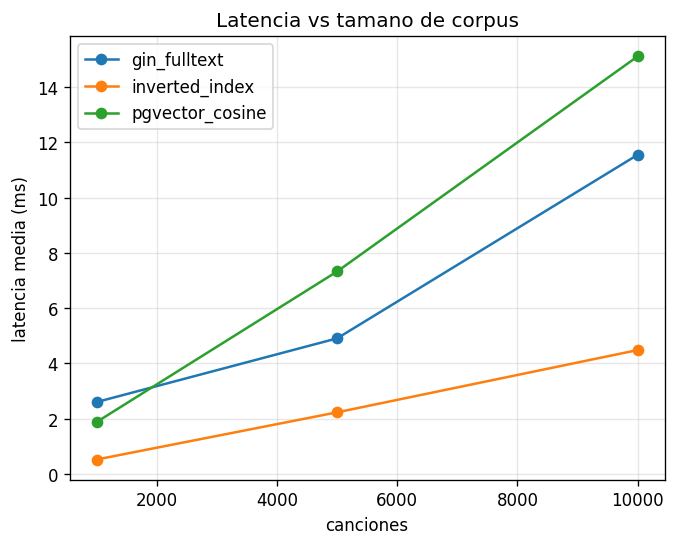
\includegraphics[width=0.48\textwidth]{latency_vs_size.png}\hfill
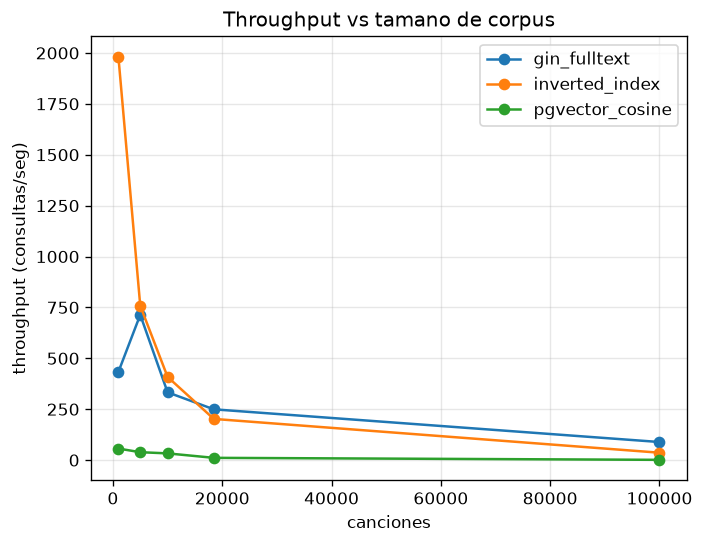
\includegraphics[width=0.48\textwidth]{throughput_vs_size.png}
\caption{Latencia (izq.) y throughput (der.) según el tamaño del corpus.}
\end{figure}

\begin{figure}[h]
\centering
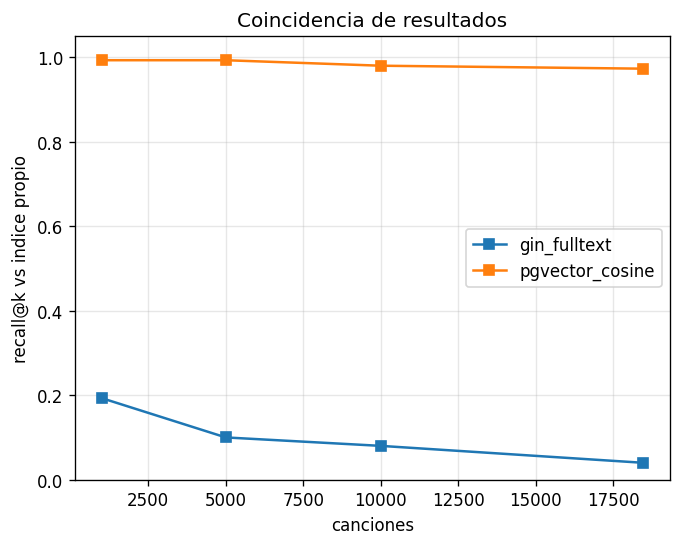
\includegraphics[width=0.48\textwidth]{recall_vs_size.png}\hfill
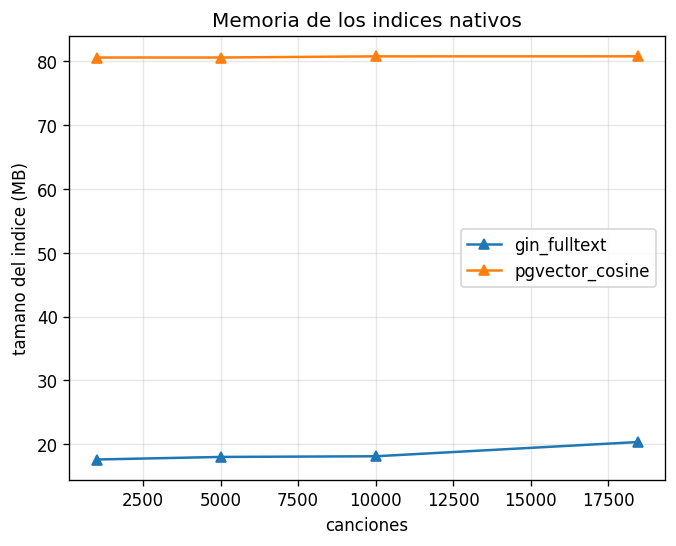
\includegraphics[width=0.48\textwidth]{memory_vs_size.png}
\caption{Recall@k (izq.) y memoria del índice nativo (der.).}
\end{figure}

\paragraph{Lectura.} El índice invertido propio es el más rápido en toda la
escala y no ocupa memoria de índice nativo (solo \textit{postings}: 71\,873
para 18\,454 chunks). \texttt{pgvector} recupera casi lo mismo que él
(recall $\approx 0.97$--$0.99$, porque ambos rankean por coseno) pero paga la
distancia densa y $\sim$80\,MB de índice. \texttt{GIN} es rápido de construir
pero su \textit{recall} frente al coseno es bajo (y \emph{cae} al crecer el
corpus): la coincidencia booleana de \textit{tokens} recupera un conjunto
distinto al del ranking por similitud --- son semánticas de consulta
diferentes, no un ``peor buscador''.

\subsection{ANN: HNSW vs.\ búsqueda exacta (pgvector)}
Aquí las dos vías corren la misma consulta coseno; lo único que cambia es si el
planner usa el índice HNSW o cae a \textit{Seq Scan} (exacto). El
\textit{recall} del aproximado se mide contra el exacto.

\begin{table}[h]
\centering
\caption{HNSW frente a búsqueda exacta, variando \texttt{ef\_search}.}
\small
\begin{tabular}{@{}lrrrr@{}}
\toprule
\textbf{Método} & \texttt{ef\_search} & \textbf{Media (ms)} & \textbf{QPS} &
\textbf{Recall@k} \\
\midrule
pgvector exacto & ---  & 54.39 & 18   & 1.00 \\
pgvector HNSW   & 10   & 0.82  & 1213 & 0.55 \\
pgvector HNSW   & 20   & 0.73  & 1364 & 0.71 \\
pgvector HNSW   & 40   & 0.97  & 1033 & 0.85 \\
pgvector HNSW   & 80   & 1.16  & 861  & 0.89 \\
pgvector HNSW   & 160  & 1.71  & 585  & 0.92 \\
\bottomrule
\end{tabular}
\end{table}

\begin{figure}[h]
\centering
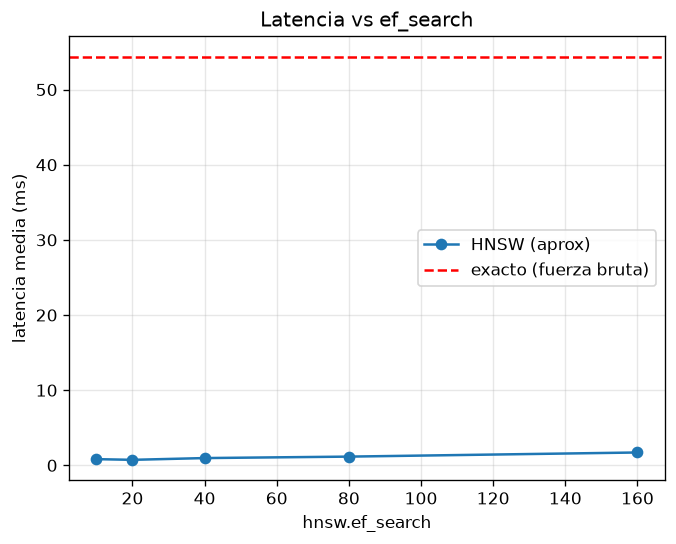
\includegraphics[width=0.48\textwidth]{ann_latency_vs_ef.png}\hfill
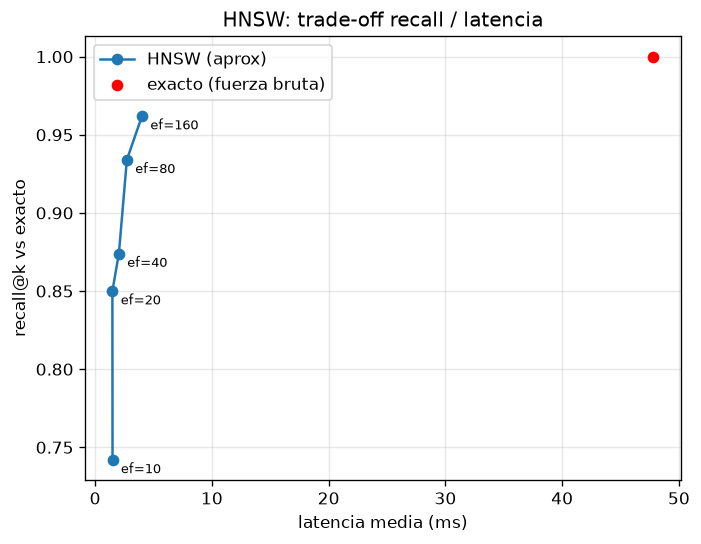
\includegraphics[width=0.48\textwidth]{ann_recall_vs_latency.png}
\caption{HNSW: latencia según \texttt{ef\_search} (izq.) y la curva
recall--latencia (der.).}
\end{figure}

\paragraph{Lectura.} HNSW es $\sim$55--75$\times$ más rápido que la búsqueda
exacta (de 54\,ms a $<$2\,ms), a costa de \textit{recall}. El parámetro
\texttt{ef\_search} controla el \textit{trade-off}: con \texttt{ef\_search}=160
se alcanza recall $0.92$ manteniendo $\sim$585 QPS. Es el ejemplo de manual de
``sacrificar exactitud por velocidad'' de la búsqueda aproximada.

\subsection{Audio: índice propio vs.\ pgvector}
Sobre las 1\,000 pistas de GTZAN, la búsqueda de similitud acústica por ambas
vías devuelve \emph{exactamente el mismo ranking con los mismos puntajes}
(ambos calculan coseno sobre los mismos histogramas de \textit{acoustic
words}). Ejemplo con la pista \texttt{blues.00000.wav} como consulta:

\begin{table}[h]
\centering
\caption{Similitud acústica: mismo top-3 por ambas vías.}
\small
\begin{tabular}{@{}lrr@{}}
\toprule
\textbf{Vecino} & \textbf{Coseno} & \textbf{Género} \\
\midrule
\texttt{rock.00071.wav}  & 0.7321 & rock \\
\texttt{blues.00059.wav} & 0.6058 & blues \\
\texttt{blues.00080.wav} & 0.5999 & blues \\
\bottomrule
\end{tabular}
\end{table}

\noindent
La latencia del índice invertido propio fue $\sim$0.4\,ms frente a
$\sim$10--12\,ms de pgvector para la misma consulta: la coincidencia exacta de
resultados con esa diferencia de costo ilustra el valor del índice invertido
compacto cuando los histogramas son dispersos.

% ---------------------------------------------------------------------------
\section{Análisis de trade-offs y conclusiones}

\begin{itemize}
  \item \textbf{¿Qué técnica ganó en qué métrica?} En \emph{latencia y memoria}
        el índice invertido propio gana en texto: es el más rápido en toda la
        escala y no requiere estructura nativa adicional. En \emph{búsqueda
        vectorial}, HNSW domina la latencia (55--75$\times$ sobre el escaneo
        exacto) al precio de \textit{recall}.
  \item \textbf{¿Se recupera la misma información?} El índice invertido y
        \texttt{pgvector} coinciden casi siempre (recall $\ge 0.97$) porque
        ambos rankean por coseno sobre el mismo histograma. \texttt{GIN}
        responde otra pregunta (coincidencia de \textit{tokens}), por eso su
        \textit{recall} contra el coseno es bajo.
  \item \textbf{Exactitud vs.\ velocidad.} La cuantización del codebook y el ANN
        introducen falsos positivos/negativos; a cambio, el sistema es
        ultra-rápido y compacto. La calidad depende de $k$ y de
        \texttt{ef\_search}.
  \item \textbf{Memoria vs.\ latencia.} pgvector es cómodo (SQL puro) pero pesa
        $\sim$80\,MB de índice; el índice invertido propio es minúsculo pero hay
        que mantener su código.
\end{itemize}

\paragraph{Limitaciones.} El histograma de texto degenera si el vocabulario es
menor que $k$; la cuantización pierde detalle fino de los descriptores; y los
índices HNSW quedan acoplados a la dimensión del codebook (hay que reindexar si
$k$ cambia).

\paragraph{Recomendaciones.} Usar el índice invertido propio como motor primario
(rápido y barato); \texttt{pgvector} + HNSW cuando se quiera delegar la búsqueda
vectorial a la base de datos; y reservar \texttt{GIN} para búsqueda literal por
palabras clave, no para similitud.

% ---------------------------------------------------------------------------
\section{Instalación y uso}

\begin{lstlisting}
# 1. Levantar todo (db + backend + frontend)
docker compose up --build           # db:5432  backend:8000  frontend:5173

# 2. Construir los indices (una vez, tras bajar los datasets a data/raw/)
python -m pipelines.ingest --app music     --modality text  --data <csv>  --k 1024 --persist
python -m pipelines.ingest --app ecommerce --modality image --data <dir>  --k 512  --persist
python -m pipelines.ingest --app music     --modality audio --data <csv>  --k 128  --persist

# 3. Usar
#   GUI:            http://localhost:5173
#   API (Swagger):  http://localhost:8000/docs
#   Health:         curl http://localhost:8000/health
\end{lstlisting}

Detalle de uso de cada aplicación y de la consola SQL multimodal en
\texttt{docs/MANUAL.md}.

\end{document}
